
\noindent\begin{minipage}{\textwidth}
    \begin{table}[H]
        \centering
        \caption{Hiperparâmetros e Resultados do Melhor Modelo - convnext\_v10\_BR\_opt\_aug}
        \vspace{0.2cm}
        \resizebox{\textwidth}{!}{%
            \begin{tabular}{ll | lrrr}
                \hline
                \multicolumn{2}{c|}{\textbf{Hiperparâmetros}} & \multicolumn{4}{c}{\textbf{Métricas por Classe}} \\ \hline
                \textbf{Parâmetro} & \textbf{Valor} & \textbf{Classe} & \textbf{Precisão} & \textbf{Recall} & \textbf{F1-Score} \\ \hline
    Agendador (Patience) & 3 & 31.2 & 0,7215 & 0,7117 & 0,7166 \\ 
Agendador de LR & ReduceLROnPlateau & 31.3 & 0,6250 & 0,5851 & 0,6044 \\ 
Architecture & convnext\_tiny & 31.4 & 0,5665 & 0,6535 & 0,6069 \\ 
Batch Size & 32 & 32.3 & 0,7220 & 0,7831 & 0,7513 \\ 
Data Augmentation & False & 32.4 & 0,7037 & 0,5278 & 0,6032 \\ 
Decaimento de Peso (WD) & 0,0482 & 33.3 & 0,7021 & 0,7639 & 0,7317 \\ 
Dropout & 0,2302 & 41.4 & 0,5926 & 0,3404 & 0,4324 \\ 
Função de Perda & CrossEntropyLoss & 41.5 & 0,6744 & 0,6744 & 0,6744 \\ 
Hidden Units & 512 & 42.4 & 0,8684 & 0,5410 & 0,6667 \\ 
Label Smoothing & 0,1192 & 44.4 & 0,8621 & 0,7812 & 0,8197 \\ 
\cline{3-6} 
Otimizador & AdamW & \textbf{Média (Macro)} & 0,7236 & 0,6547 & 0,6727 \\ 
Taxa de Aprendizado (LR) & 2,35e-04 & \textbf{MCC} & \multicolumn{3}{c}{0,6334} \\ 
Unfreeze Layers & 5 &  & & &  \\ 
            \hline
            \end{tabular}%
        }
    \end{table}

    \begin{figure}[H]
        \centering
        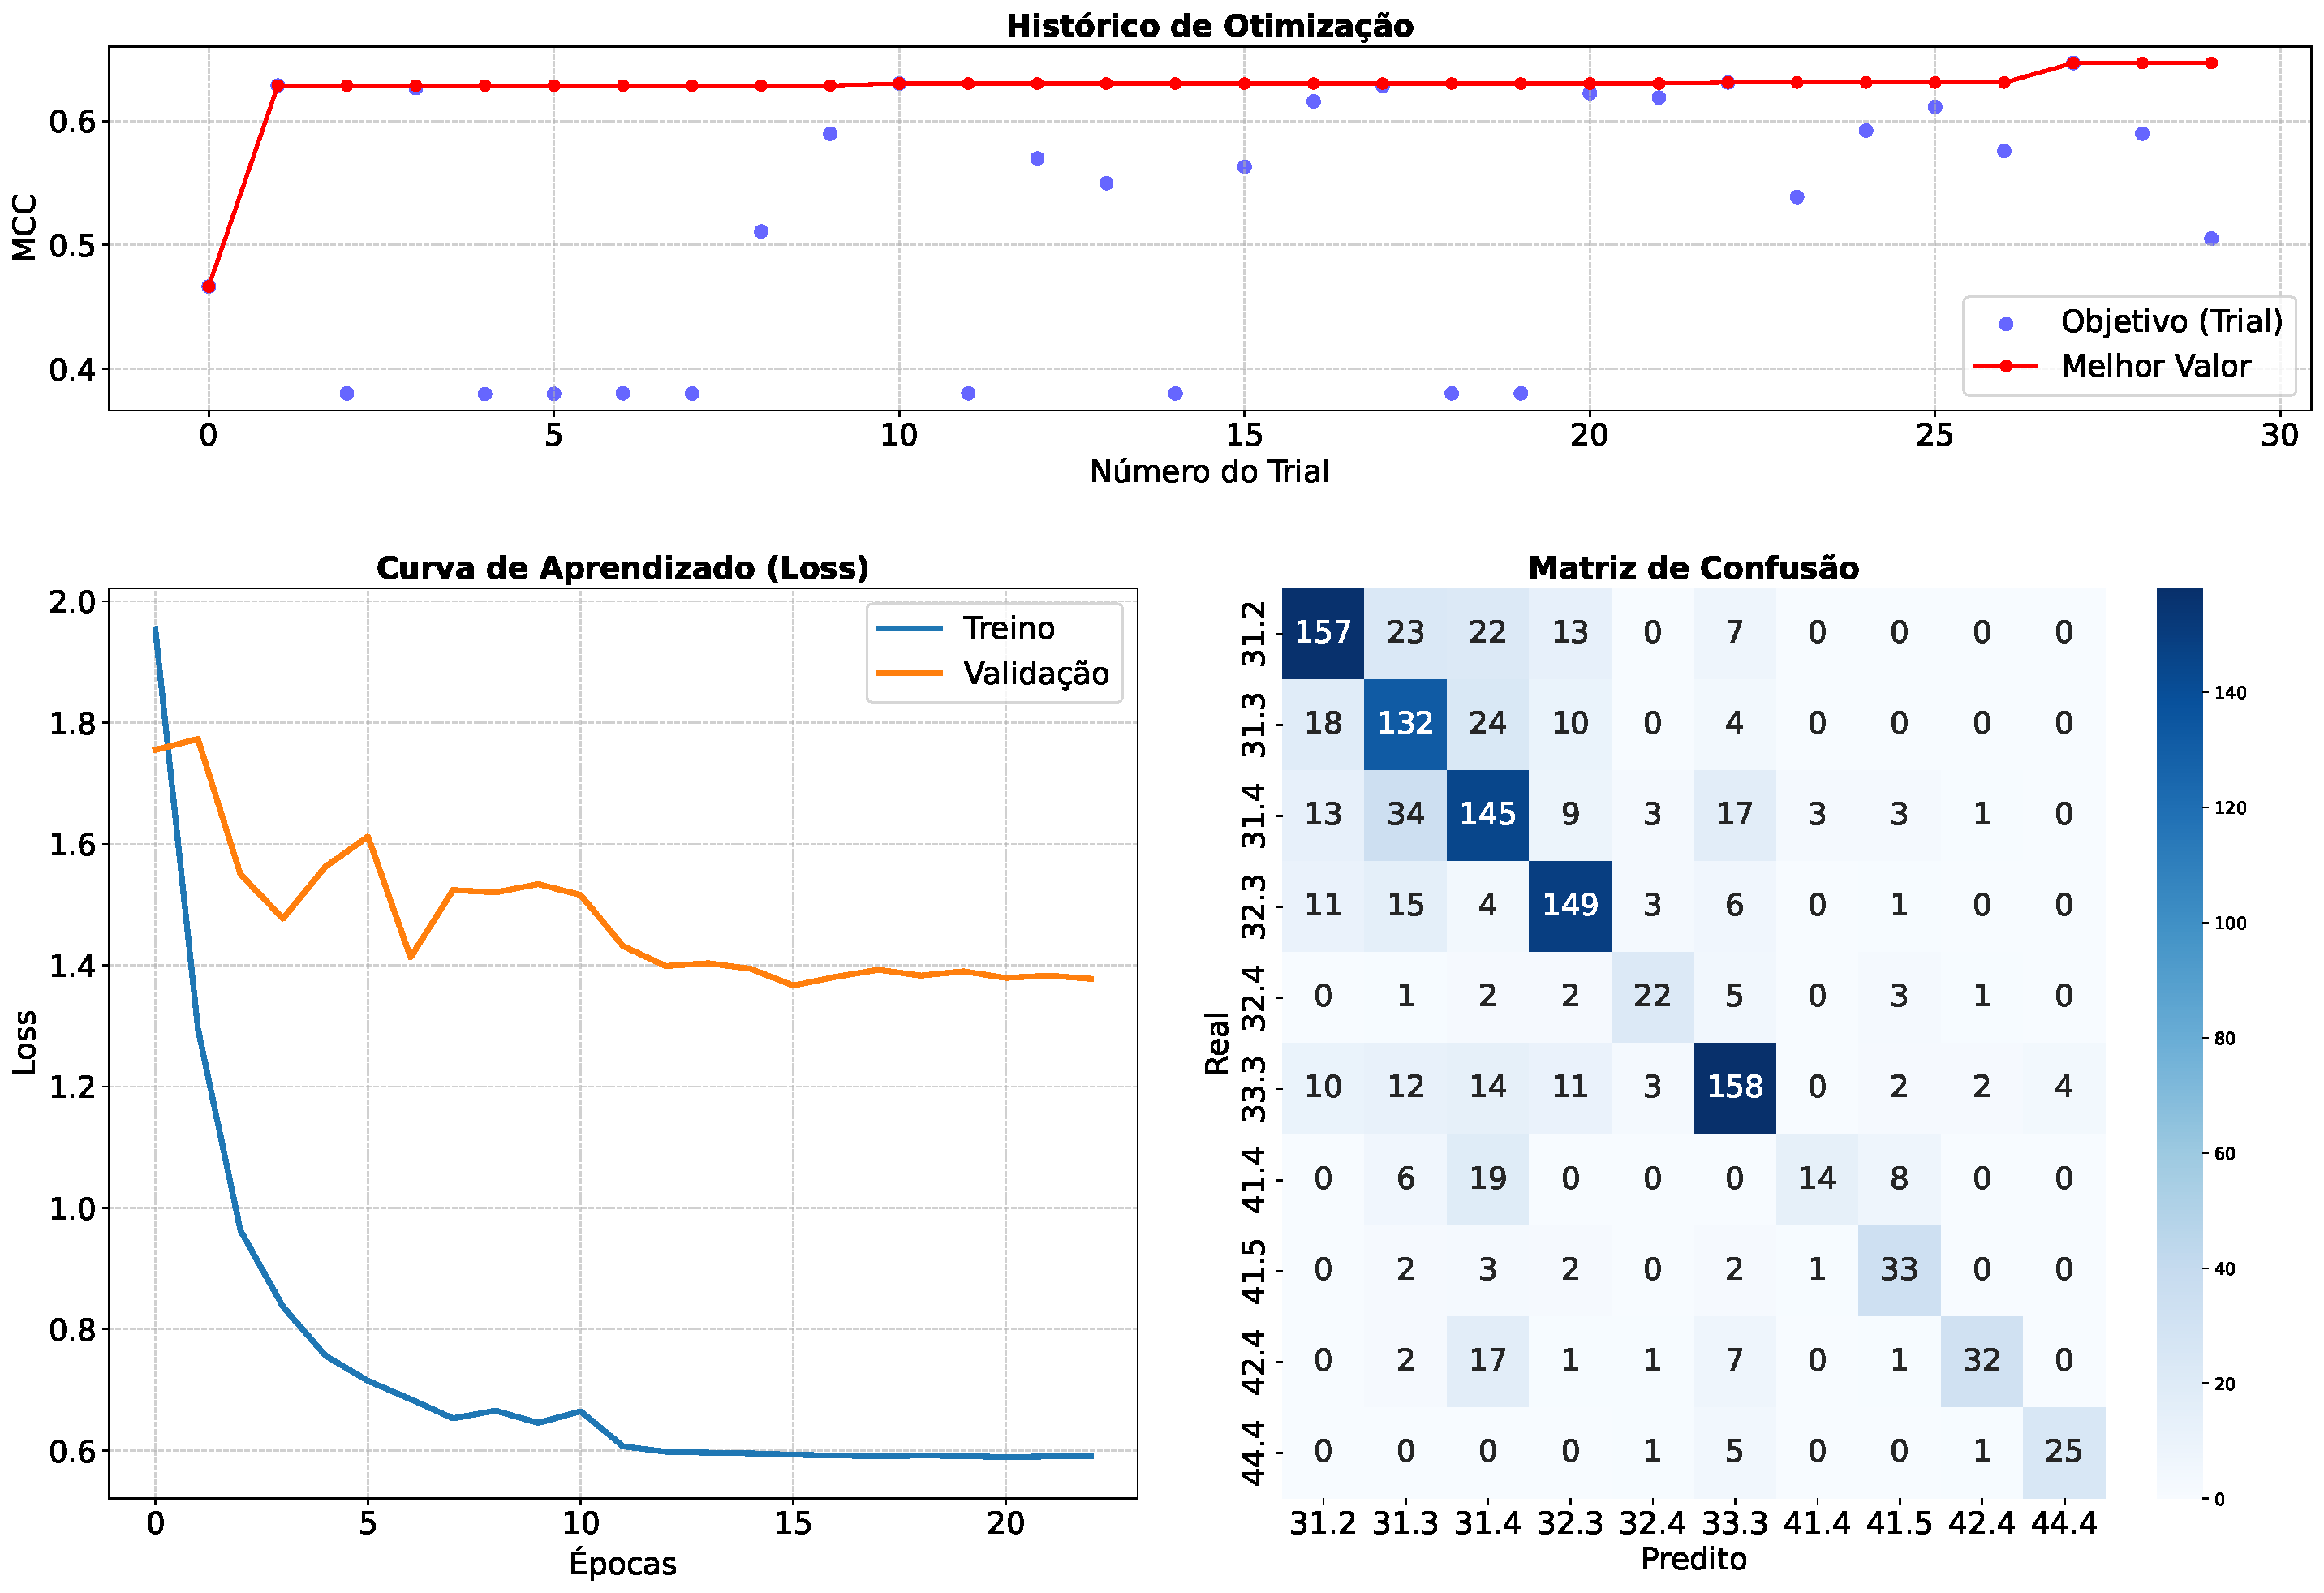
\includegraphics[width=0.85\textwidth]{tex/appendix/experiments/convnext_v10_BR_opt_aug/dashboard_consolidado.pdf}
        \caption{Histórico de Otimização, Curvas de Aprendizado e Matriz de Confusão - convnext\_v10\_BR\_opt\_aug}
    \end{figure}
\end{minipage}
\clearpage
